\chapter{Resultados y análisis}

Como se mencionó anteriormente, se implementaron tres algoritmos diferentes (RA1, LRDEA y GA-Nuggets) sobre los datos obtenidos de tres autómatas celulares diferentes (AC Brain, AC Byl, AC Evoloops y AC Mite). Para cada uno de los experimentos realizados con los autómatas celulares, se utilizaron los siguientes parámetros:

\begin{itemize}
	\item \textbf{Vecindario:} de tipo Moore con 8 vecinos.
	\item \textbf{Parámetros de GA-Nuggets:}
	\begin{itemize}
		\item $w1=1$ 
		\item $w2=2$ 
		\item $\beta=2$ 
		\item $pMutacion=0.05$
		\item $noHijos=2$ 
		\item $poblacion=100$ 
		\item $noIteraciones=100$
		\item $maximoAntecedente=50$
		\item $minimoAntecedente=3$
	\end{itemize}
	\item \textbf{Parámetros de LRDEA:}
	\begin{itemize}
		\item $noHijos=2$
		\item $poblacion=100$
		\item $pMutacion=0.05$
		\item $noIteraciones=100$
	\end{itemize}
	\item \textbf{Parámetros de RA1:}
	\begin{itemize}
		\item $l=5$
	\end{itemize}
\end{itemize}

No está de más mencionar que la naturaleza del algoritmo RA1 requiere de menos parámetros definidos como los algoritmos anteriores porque este algoritmo depende menos de factores aleatorios.


\section{Brain}
En las figuras \ref{fig:ra1brain}, \ref{fig:lrdeabrain} y \ref{fig:ganuggetsabrain} se muestran los resultados de exactitud de los tres algoritmos implementados en los datos del AC Brain. Estos resultados se muestran a partir del estado 160 y hasta el estado 200 debido a que estos son los estados en los que se calculan los errores de aprendizaje y generalización (datos amarillos y rojos del diagrama de la figura \ref{fig:walkforward}), mientras que los datos previos (azules) son utilizados para el entrenamiento.
\\
Como se puede observar en la figura \ref{fig:ra1brain} el algoritmo RA1 tuvo un muy buen desempeño con un promedio de exactitud de 89\% dentro del conjunto de datos y de 85\% en fuera del conjunto  a comparación del algoritmo LRDEA (figura \ref{fig:lrdeabrain}) que obtuvo un promedio de 88\% y 81\% respectivamente y el algoritmo GA-Nuggets con 88\% y 79\% (figura \ref{fig:ganuggetsabrain}).

	\begin{figure}[H]
		\centering
		\includegraphics[width=\linewidth]{fig/ra1_0}
		\caption{Exactitud de el algoritmo RA1 sobre el conjunto de datos del AC Brain.}
		\label{fig:ra1brain}
	\end{figure}

	\begin{figure}[H]
		\centering
		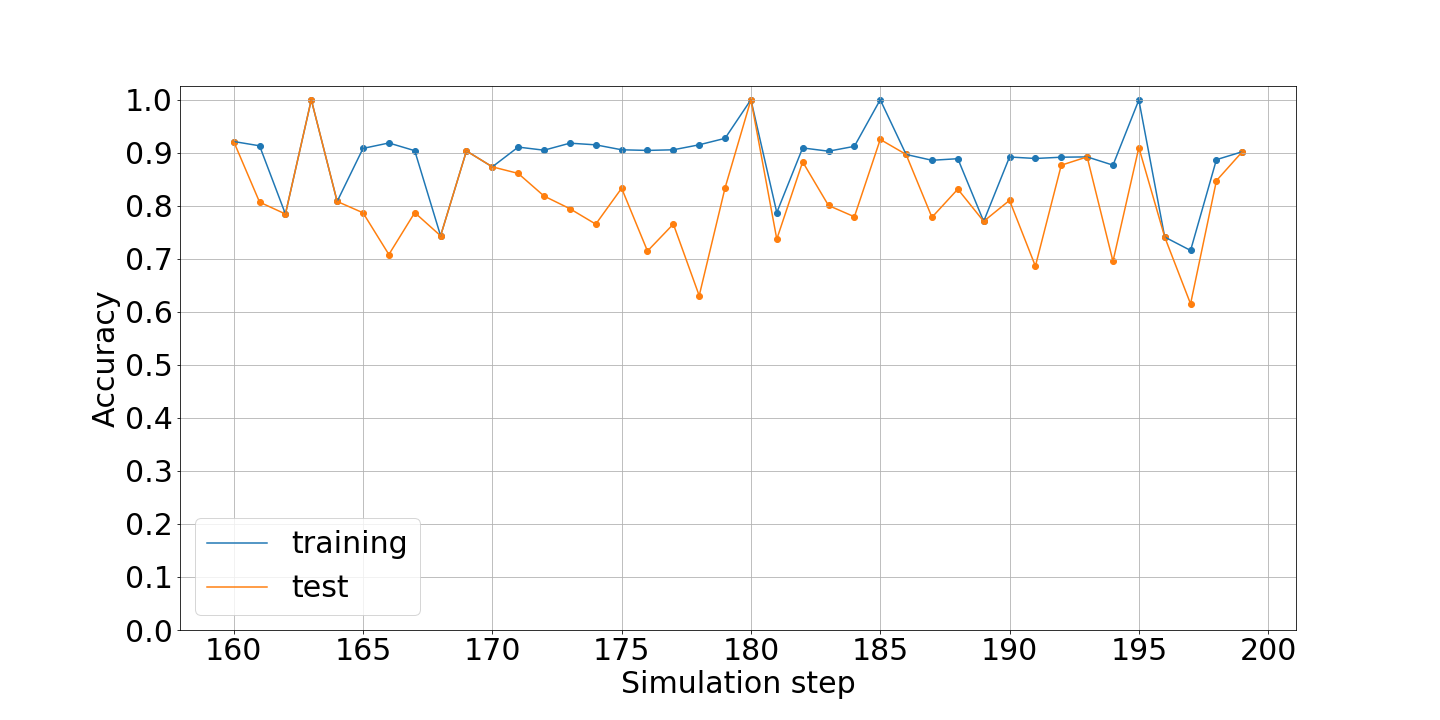
\includegraphics[width=\linewidth]{fig/LRDEA_1}
		\caption{Exactitud de el algoritmo LRDEA sobre el conjunto de datos del AC Brain.}
		\label{fig:lrdeabrain}
	\end{figure}

	\begin{figure}[H]
		\centering
		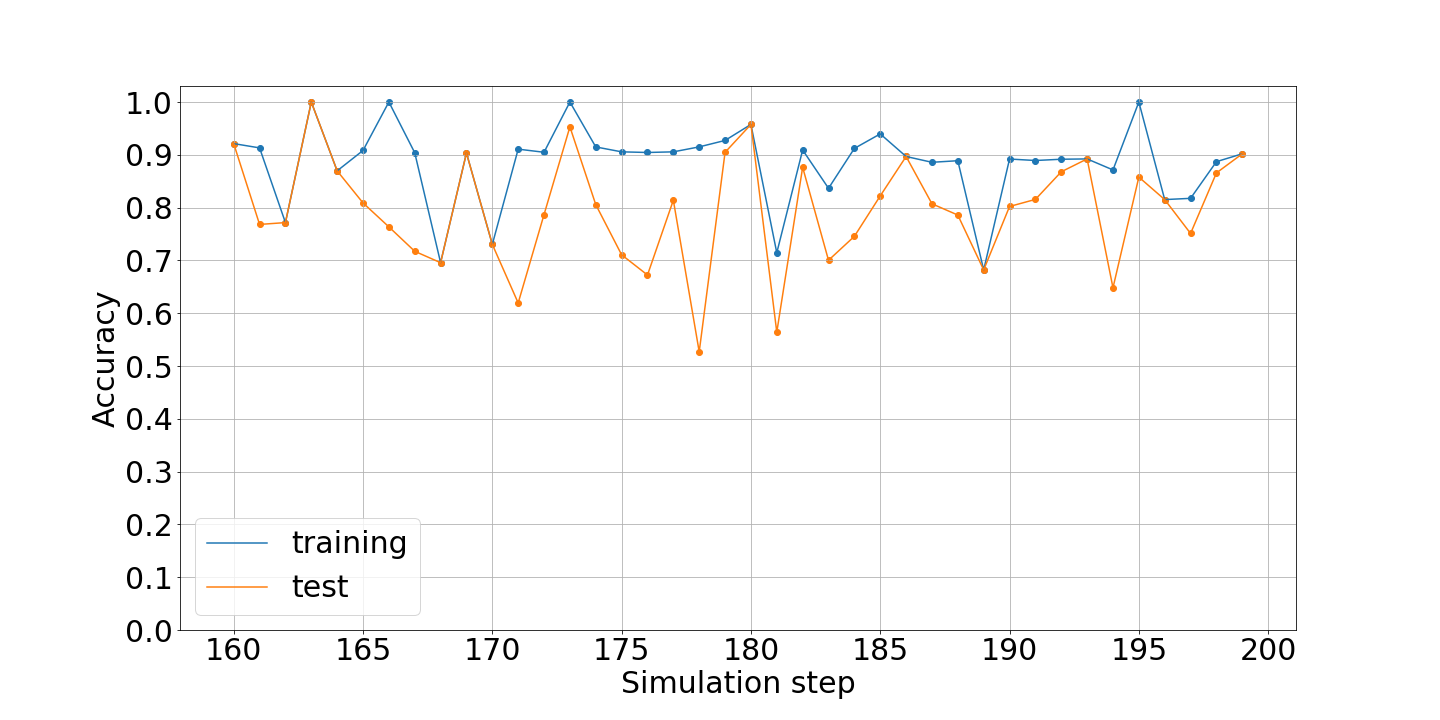
\includegraphics[width=\linewidth]{fig/GA-nuggets_2}
		\caption{Exactitud de el algoritmo GA-Nuggets sobre el conjunto de datos del AC Brain.}
		\label{fig:ganuggetsabrain}
	\end{figure}

\section{Byl}
De manera similar a la presentación de los resultados anteriores, en las figuras \ref{fig:ra1byl}, \ref{fig:lrdeabyl} y \ref{fig:ganuggetsabyl} se muestran los resultados de exactitud de los tres algoritmos implementados en los datos del AC Byl.

Como se logra apreciar en las figuras a continuación, en ciertos estados se logró obtener una exactitud del 100\%, esto es debido a que ciertos estados tienen un comportamiento más trivial que los otros, lo que resulta más fácil de aprender para los algoritmos.
\\
De la misma forma que los resultados para los datos del AC Brain, el algoritmo que obtuvo mejor valor de exactitud fue el RA1 con un promedio de 90\% en el conjunto de entrenamiento y un 85\% fuera del conjunto de entrenamiento. A su vez, el algoritmo LRDEA obtuvo un promedio de 91\% y 84\% , lo que nos indica que el algoritmo tiene más variación con respecto al RA1. Por último, el algoritmo GA-Nuggets obtuvo 89\% y 77\% con mayor variación y menor valor de exactitud con respecto a los otros dos algoritmos.
\begin{figure}[H]
	\centering
	\includegraphics[width=\linewidth]{fig/ra1_3}
	\caption{Exactitud de el algoritmo RA1 sobre el conjunto de datos del AC Byl.}
	\label{fig:ra1byl}
\end{figure}

Es interesante notar cómo en la figura \ref{fig:lrdeabyl} y la figura \ref{fig:ganuggetsabyl} se ve un comportamiento similar, a comparación con la figura \ref{fig:ra1byl}. Esto puede deberse a las dinámicas que rigen a los algoritmos genéticos, se podría esperar que el algoritmo RA1 sea menos propenso a variaciones por que depende en menor medida de la probabilidad.
\begin{figure}[H]
	\centering
	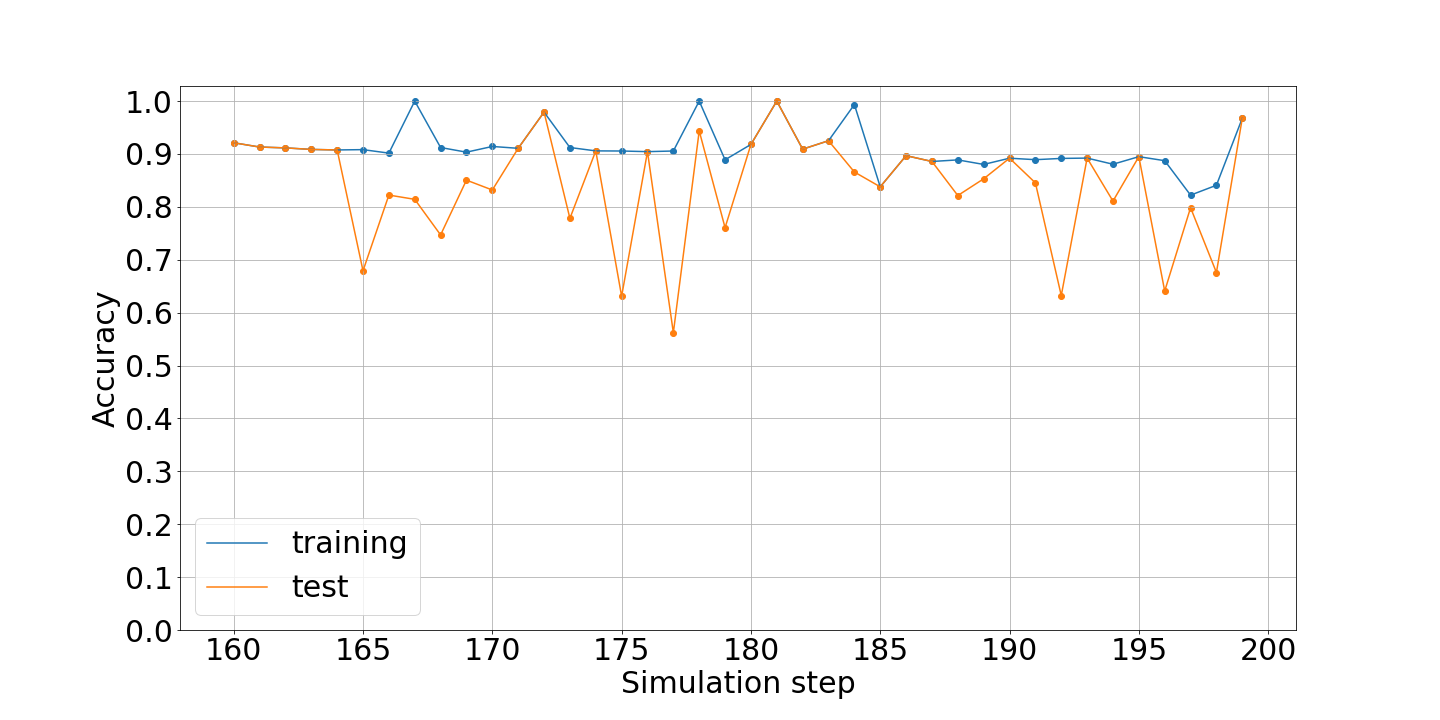
\includegraphics[width=\linewidth]{fig/LRDEA_4}
	\caption{Exactitud de el algoritmo LRDEA sobre el conjunto de datos del AC Byl.}
	\label{fig:lrdeabyl}
\end{figure}

\begin{figure}[H]
	\centering
	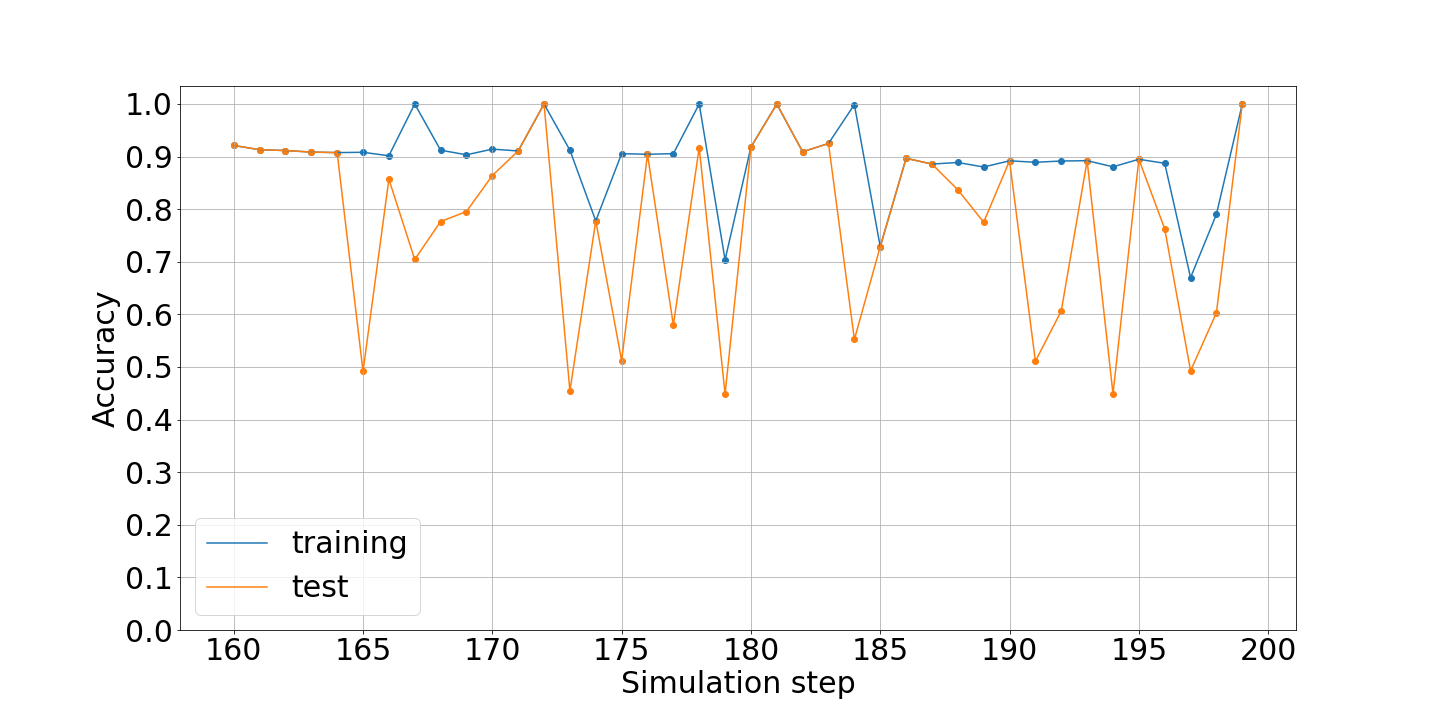
\includegraphics[width=\linewidth]{fig/GA-nuggets_5}
	\caption{Exactitud de el algoritmo GA-Nuggets sobre el conjunto de datos del AC Byl.}
	\label{fig:ganuggetsabyl}
\end{figure}

\section{Evoloops}
Al igual que con Byl este experimento fue uno en los cuales se obtuvo mejor desempeño, con un promedio de 90\% de exactitud dentro del entrenamiento y 86\% fuera de entrenamiento, el algoritmo RA1 fue el que obtuvo la mejor exactitud. En segundo lugar, se encuentra el algoritmo LRDEA con 89\% y 82\% y, por último, el algoritmo GA-Nuggets con 88\% y 78\%.
\begin{figure}[H]
	\centering
	\includegraphics[width=\linewidth]{fig/ra1_6}
	\caption{Exactitud de el algoritmo RA1 sobre el conjunto de datos del AC Evoloops.}
	\label{fig:ra1evoloops}
\end{figure}
\begin{figure}[H]
	\centering
	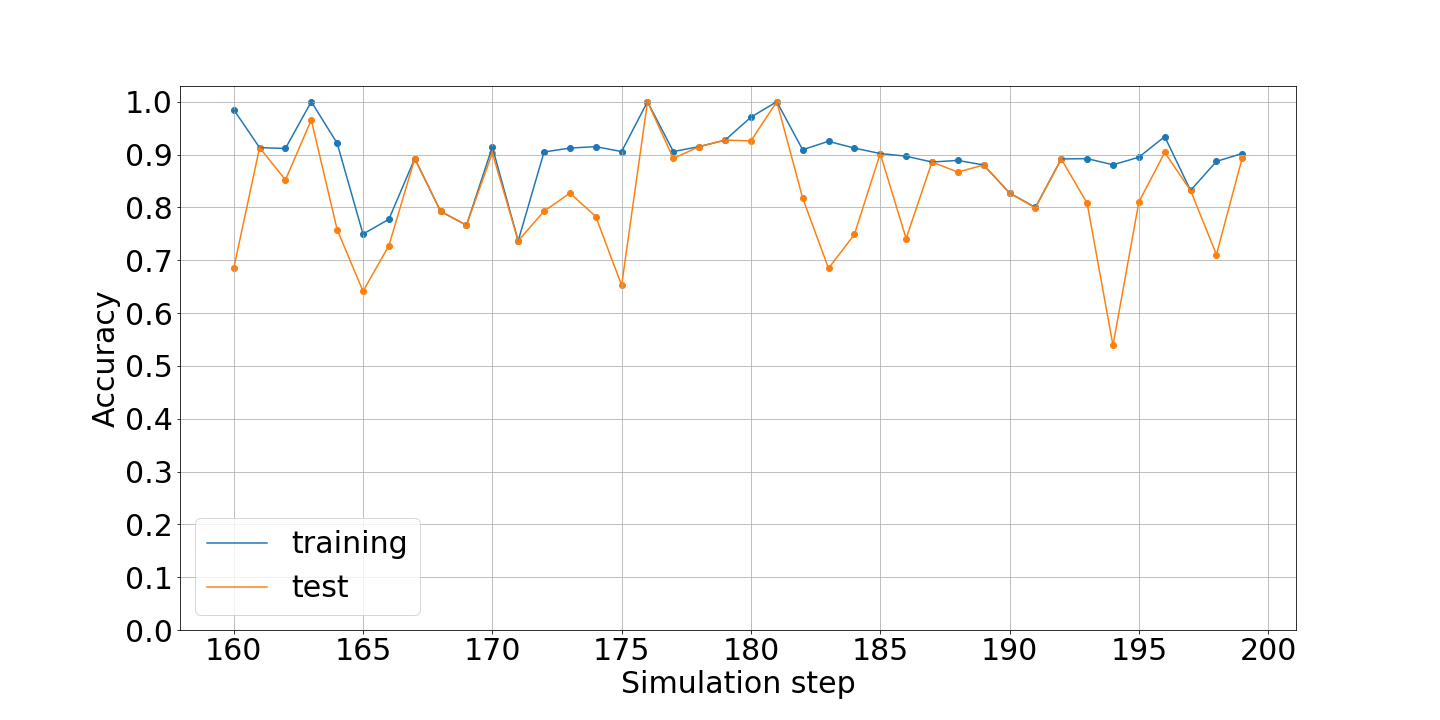
\includegraphics[width=\linewidth]{fig/LRDEA_7}
	\caption{Exactitud de el algoritmo LRDEA sobre el conjunto de datos del AC Evoloops.}
	\label{fig:lrdeaevoloops}
\end{figure}

En la siguiente gráfica se puede observar cómo el GA-Nuggets puede tener mucha variación en su exactitud, en comparación a los otros dos algoritmos.

\begin{figure}[H]
	\centering
	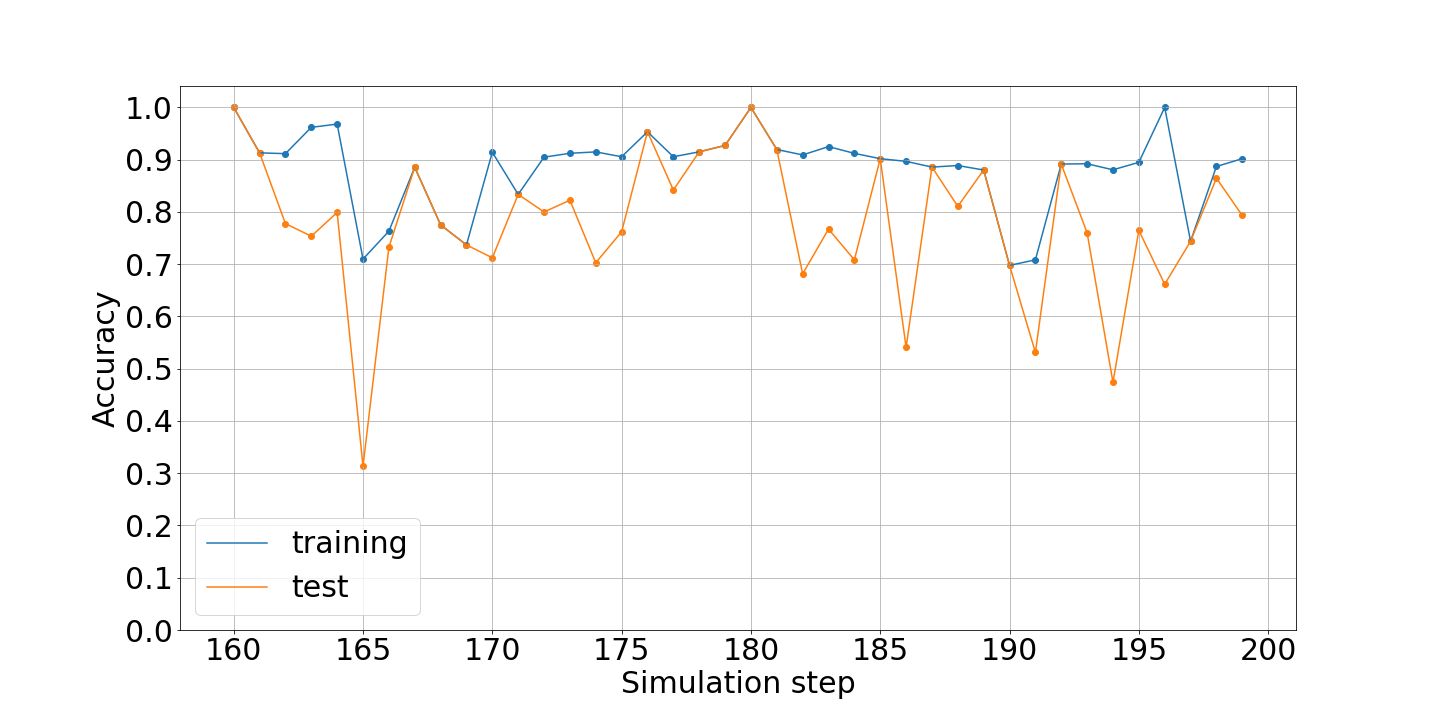
\includegraphics[width=\linewidth]{fig/GA-nuggets_8}
	\caption{Exactitud de el algoritmo GA-Nuggets sobre el conjunto de datos del AC Evoloops.}
	\label{fig:ganuggetsevoloops}
\end{figure}

\section{Mite}
En este experimento, fue en el que se obtuvieron los resultados más bajos, sin embargo, aun así logramos ver que la propuesta (LRDEA) sigue siendo capaz de mantenerse a un buen nivel, en comparación con los otros dos algoritmos.

Los promedios de exactitud dentro y fuera de entrenamiento para los datos del AC Mite, son los siguientes: RA1 con 89\% y 84\%, LRDEA con 89\% y 81\%, y por último GA-Nuggets con 88\% y 75\%, respectivamente.

\begin{figure}[H]
	\centering
	\includegraphics[width=\linewidth]{fig/ra1_9}
	\caption{Exactitud de el algoritmo RA1 sobre el conjunto de datos del AC Mite.}
	\label{fig:ra1mite}
\end{figure}
\begin{figure}[H]
	\centering
	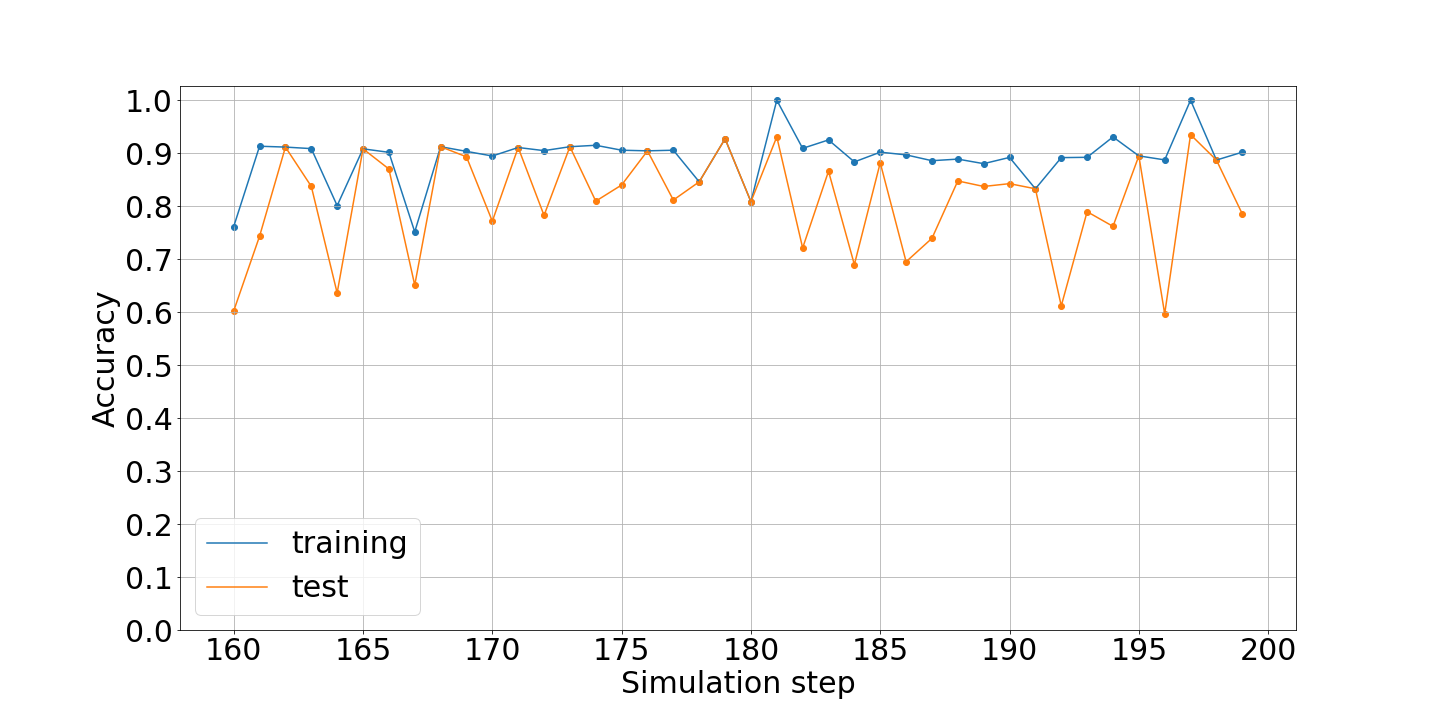
\includegraphics[width=\linewidth]{fig/LRDEA_10}
	\caption{Exactitud de el algoritmo LRDEA sobre el conjunto de datos del AC Mite.}
	\label{fig:lrdeamite}
\end{figure}

\begin{figure}[H]
	\centering
	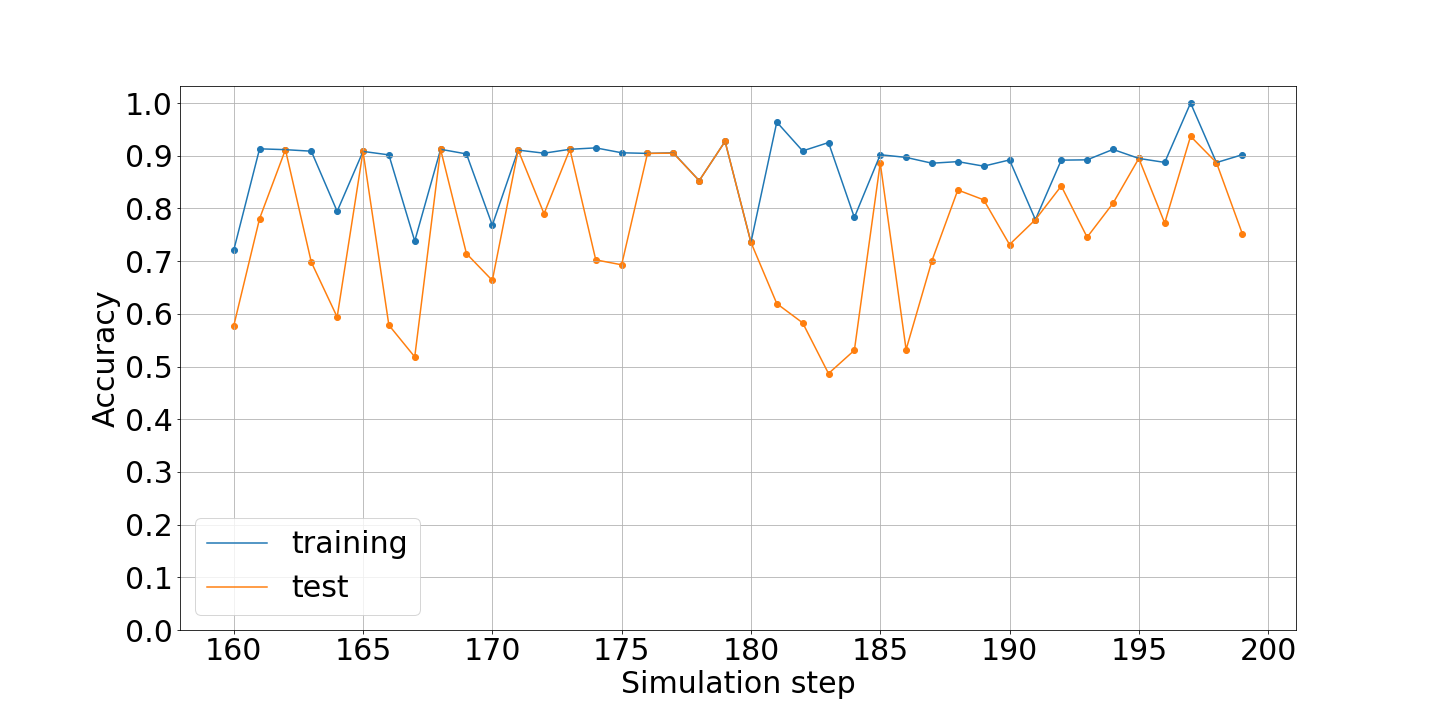
\includegraphics[width=\linewidth]{fig/GA-nuggets_11}
	\caption{Exactitud de el algoritmo GA-Nuggets sobre el conjunto de datos del AC Mite.}
	\label{fig:ganuggetsmite}
\end{figure}